\newcommand{\etas}{\ensuremath{\eta_{\mathrm{s}}}}


\chapter{Preliminaries}
\section{Jaynes Cummings Model}
To better understand the Jaynes Cummings Model, it is instructive to consider the case of a single qubit or two level atom in a perfect non leaky cavity.
\citep{gerry2005introductory}

%\textbf{cite gerry chp 4, 4.5} 
\begin{figure}
\centering
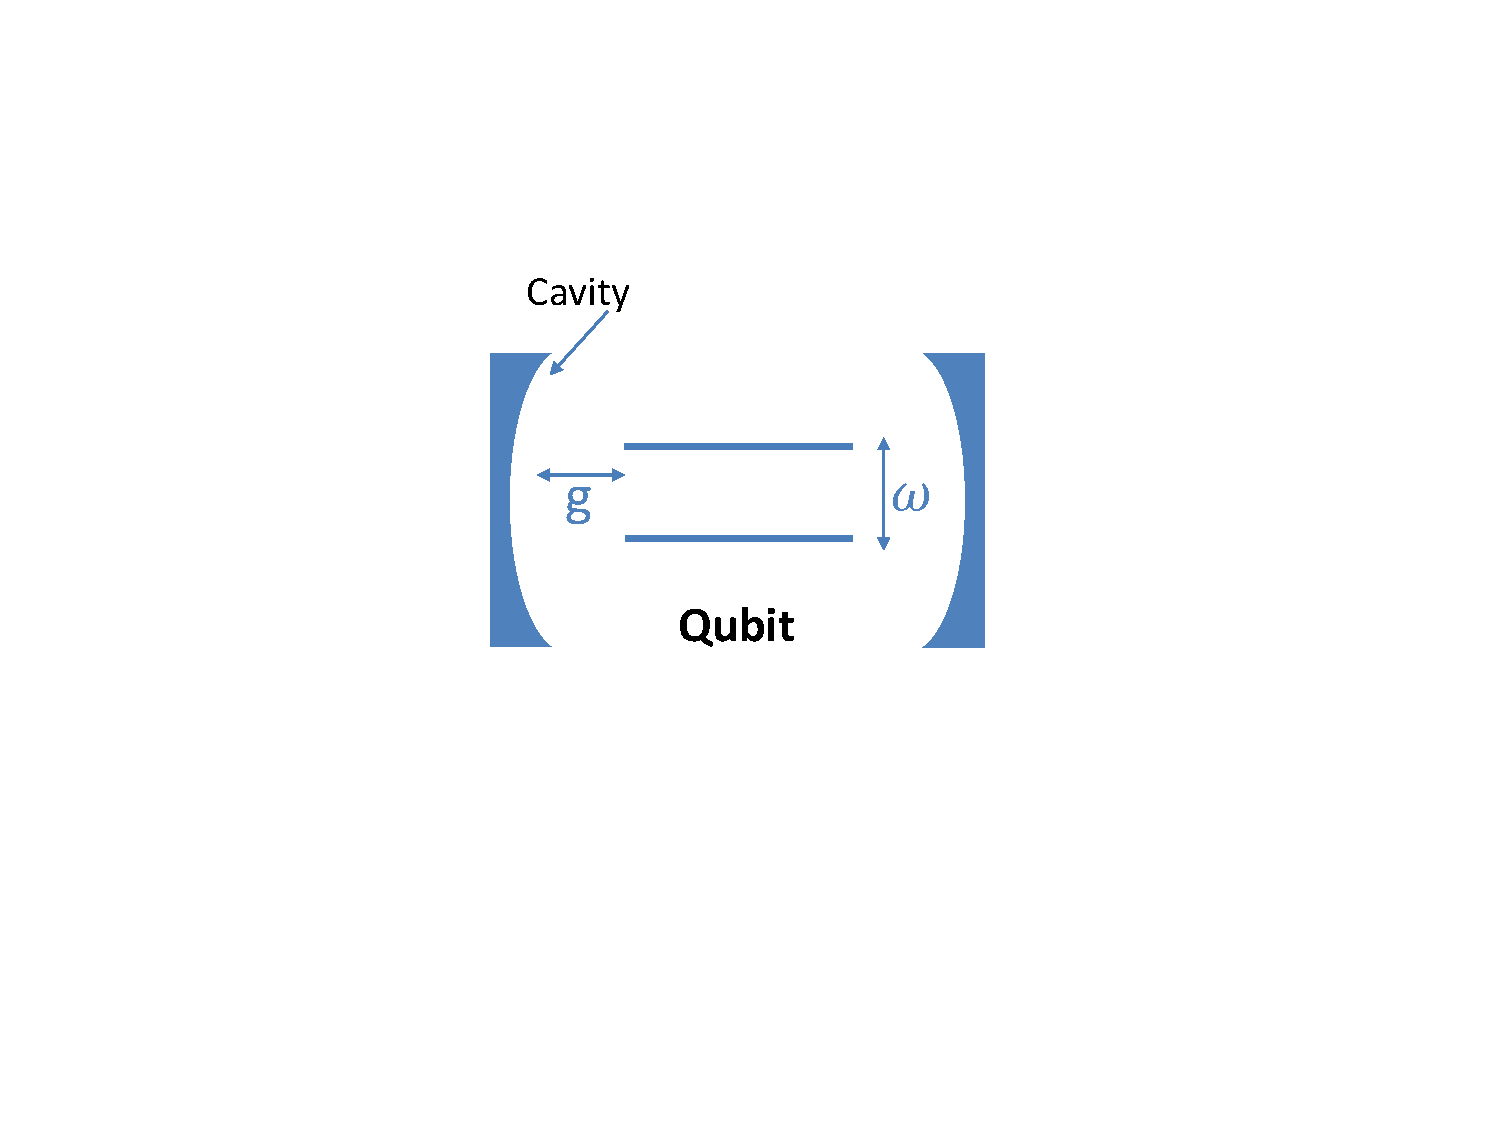
\includegraphics[width=0.5\textwidth]{Figr2a.pdf}
\caption{Single qubit in a perfect non leaky cavity}
\label{fig:Figr2a}
\end{figure}

Let the lower level be $\ket{g}$ and the upper level be $\ket{e}$. These two levels would be in contact with a electric field in the cavity. The cavity electric field in a quantized form is given by: 

%\begin{center}
\begin{align}\label{eq:3}
\hat { E } &=\hat{e}{ \left( \frac { \hslash \Omega  }{ { \epsilon  }_{ 0 }V }  \right)  }^{ { 1 }/{ 2 } }\left( {  a _{-} }+{  a  }_{ +  } \right) \sin { \left( kz \right) }
\end{align}
%\end{center}
%\textbf{cite gerry chp 2, 2.1}\\

The interaction Hamiltonian would be the following format effectively.
%\begin{center}
\begin{align}\label{eq:4}
{ H  }^{ \left( I \right)  }&= -\hat{D} {.} \hat{E}  \\
&=d g\left( {  a_{-}  }+{  a  }_{ +  } \right)
\end{align}
%\end{center}

where $ d $ = dipole moment operator of the atom, $\hat{D}$ is the dipole moment vector,%\\ 
%\textbf{cite gerry chp 4, 4.1}\\

%where
%\begin{center}
\begin{align}\label{eq:5}
g &= -{ \left( \frac { \hslash \Omega  }{ { \epsilon  }_{ 0 }V }  \right)  }^{ { 1 }/{ 2 } } \sin { \left( kz \right) }
\end{align}
%\end{center}

and  $ d = \hat{D}. \hat{e}$. At this point it is convenient to introduce the so-called atomic transition
operators.


%\begin{center}
\begin{align}\label{eq:7}
\sigma_{+}&=\dyad{e}{g},\quad \sigma_{-}= \dyad{g}{e}=\sigma_{+}^{ \dagger  },
\end{align}
%\end{center}\ket{e}\bra{g} \ket{g}\bra{e}
and the inversion operator 
%\begin{center}
\begin{align}\label{eq:8}
\sigma_{3}&=\dyad{e}-\dyad{g}.
\end{align}
%\end{center}\ket{g}\bra{g}
%$\bra{2} \ket{2} \braket{10} \dyad{e}{g}$
These operators obey the Pauli spin algebra
\begin{align}\label{eq:9}
[\sigma_{+},\thinspace\sigma_{-}] &=\sigma_{3}\\ %\notag
[\sigma_{3},\thinspace\sigma_{\pm}] &=2\sigma_{\pm}.
\end{align}

By parity, one can say that, the diagonal elements of ${d} = {0}$. Symmetry conditions coerce an atom to have a net zero dipole movement, if it is in an energy eigenstate. Hence the diagonal elements of ${d}$  would be zero $\expval{d}{e} = 0 = \expval{d}{g} $, 
%${d} = {0}$ This is also evident.

%\begin{center}
\begin{align}\label{eq:9.1}
\begin{split}
d&= d\dyad{g}{e}+{d}^{*}\dyad{e}{g}\\ 
&=d\sigma_{-} + d^{*}\sigma_{+} = d(\sigma_{+} + \sigma_{-}) 
\end{split}
\end{align}
%\end{center}\ket{g}\bra{e} \ket{e}\bra{g}
%d&= d\dyad{g}{e}+{d}^{*}\dyad{e}{g}\\ 
%&=d\sigma_{-} + d^{*}\sigma_{+} =d(\sigma_{+} + \sigma_{-}) \notag
where we have set $\mel{e}{d}{g}$ = d and have assumed, without loss of generality, that d is real. Thus the interaction Hamiltonian is %\eqref{eq:9.1}

%\begin{center}
\begin{align}\label{eq:10}
H^{(I)}&= \hslash\lambda(\sigma_{+} + \sigma_{-})({a}_{-} + {a}_{+})
\end{align}
%\end{center}
where $\lambda=dg/\hslash $%\newpage

\subsubsection{Derivation of the time dependence of the operators}
The explanation below closely follows that in chapter 2, section 2.1 of \citep{gerry2005introductory}.
The Hamiltonian of a harmonic oscillator is given by 
\begin{align}\label{eq:10.1}
H &=\hslash \Omega \left( { a}_{+  }a_{-} +\frac { 1 }{ 2 }  \right)
\end{align}
The Heisenberg equation for operators reads as
\begin{align}\label{eq:10.2}
\frac { d O  }{ dt } &=\frac { i }{ \hslash  } \left[ H ,O  \right] 
\end{align}

On substituting for the annihilation operator $a_{-}$ one gets
\begin{align}\label{eq:10.3} %\label{bch}
\frac { da_{-}  }{ dt } &=\frac { i }{ \hslash  } \left[ H ,a_{-}  \right]\notag\\
&=\frac { i }{ \hslash  }\left[\hslash \Omega \left( { a}_{+  }a_{-} +\frac { 1 }{ 2 }  \right),a_{-}\right]\\
&=i\Omega \left( { a}_{+  }a_{-}a_{-} -a_{-}{ a}_{+  }a_{-}  \right)\notag\\ 
&=i\Omega \left[{a}_{-},{{a}}_{+}\right]{a_{-}}=-i\Omega {a_{-}},\notag 
\end{align}

which has the solution
\begin{align}\label{eq:10.4}
{a}_{-}(t)&={a}_{-}(0){ e }^{ -i\Omega t }\\
{a}_{+}(t)&={a}_{+}(0){ e }^{  i\Omega t }
\end{align}

%\begin{align}

%\end{align}
Another way of doing it would be via the Baker-Hausdroff lemma \citep{sakurai1995modern}
For any two operators ${A} \thinspace $ and $\thinspace B,$

\begin{align}\label{eq:10.5}
{e }^{ i\lambda A  }B { e }^{ -i\lambda A }=B+{i}\lambda\left[A,B\right]+\frac{{\left(i\lambda  \right)}^{2}}{2!}\left[A\left[A,B\right]\right]+\dots
\end{align}

The solution to \eqref{eq:10.2} can be written as
\begin{align}\label{eq:10.6}
O(t)&={ e }^{ iH t/\hslash  }O (0){ e }^{ -iH t/\hslash  }
\end{align}


Applying it to \eqref{eq:10.6} with $a_{-}$ as $H$, $\lambda$ as $t/\hslash$ and  $B$ as $O (0)$ we get,
 \begin{align}\label{eq:10.7}
 O(t)&=O(0)+\frac { it }{ \hslash  } \left[ H ,O (0) \right]\notag \\ 
&+\frac { 1 }{ 2 !}\left(\frac { it }{ \hslash} \right)^{2}\left[H,\left[H,O(0)\right]\right]+......\notag\\
&+\frac { 1 }{ n !}\left(\frac { it }{ \hslash} \right)^{n}\left[H,\left[H,\left[H,....\left[H,O(0)\right]\right]\right]\right]+......
 \end{align}

Replacing $O$ by $a_{-}$ one obtains
\begin{align}\label{eq:10.8}
a_{-} (t)&=a_{-} (0)\left[ 1-i\Omega t-\frac { { \Omega  }^{ 2 }{ t }^{ 2 } }{ 2! } +i\frac { { \Omega  }^{ 3 }{ t }^{ 3 } }{ 3! } +........ \right] \notag \\
&=a_{-} (0){ e }^{ -i\Omega t }
\end{align}


%\newpage
Writing the evolution of operators once again,(just to avoid confusion)
%These can be derived by  either Baker Hausdorff lemma as shown in 
%\textbf{cite gerry chp 2, 2.1}   
%\begin{center}
%\end{center}
\begin{align}\label{eq:11}
a_{-}(t)&=a_{-}(0){e}^{-i{\Omega}t}\\ \notag 
a_{+}(t)&=a_{+}(0){e}^{i{\Omega}t}
\end{align}

Similarly,  the time evolution of the operators for the free-atomic case is as follows
\begin{align}\label{eq:12}
\sigma_{\pm}(t)&=\sigma_{\pm}(0){e}^{\pm{i}{\omega}t}
\end{align}
%\begin{center}
%\end{center}

expanding \eqref{eq:10} we have %equation ${2.11}$
\begin{align}\label{eq:13}
H^{(I)}&= \hslash\lambda(\sigma_{+} {a}_{-} + \sigma_{+}a_{+} + \sigma_{-} a_{-} + \sigma_{-}a_{+} )
\end{align}
%\begin{center}
%\end{center}

Let us look at approximate time dependencies for each of term in above mentioned equation. Using \eqref{eq:12} and \eqref{eq:11} one can compute the time dependence of each of the terms in the bracket in \eqref{eq:13}. Thus we can see that the approximate time dependences of the operator products
in ~\eqref{eq:13} are as follows:

%\begin{center}
\begin{align}\label{eq:14}
\sigma_{+}a_{-}\quad{\sim}\quad {e}^{i({\Omega}-{\omega})t}\\ 
\sigma_{+}a_{+}\quad{\sim}\quad {e}^{i({\omega}+{\Omega})t}\\
   \sigma_{-}a_{-}\quad{\sim}\quad {e}^{-i({\omega}+{\Omega})t}\\
\sigma_{-}a_{+}\quad{\sim}\quad {e}^{-i({\Omega}-{\omega})t} 
\end{align}
%\end{center}

If the electric field frequency  in the cavity is not quite detuned  from the spacing between the energy levels of the qubits then ${\Omega}$  is quite close to ${\omega}$. Hence  ${\omega} +  {\Omega} $ is very much larger than ${\omega} -  {\Omega} $ ( because ${\Omega} \approx  {\omega} $). On time averaging the Hamiltonian in \eqref{eq:13} the contribution of the middle two terms  becomes negligibly small if the above conditions hold. Since these terms oscillate very rapidly, on integration  they get multiplied with a pre-factor which is quite huge as compared to first two terms.  Hence they can be neglected. This approximation is also called as Rotating Wave Approximation (RWA). On carrying out RWA on \eqref{eq:13} it transforms to 


\begin{center}
\begin{align}\label{eq:15}
\hat{H}^{(I)}&= \hslash\lambda(\sigma_{+} a_{-}  + \sigma_{-}a_{+} )
%\hat{H}^{I} &=\hslash\lambda(\sigma_{+}  + \sigma_{-}a_{+})(\hat{a} + })
\end{align}
\end{center}


\section{Differential equation  governing time evolution}
\subsection{Closed vs.\ open quantum systems}
When one begins to learn quantum mechanics, it is implicitly assumed that all the systems that one studies exist in isolation. This is to say that they have no interaction with any other systems. In effect, all these system assumed to be closed and hence they are known as closed quantum systems. The system that we have here (i.e. two qubits in a leaky cavity ) dissipates energy into the environment. Thus it is an open system in contrast to  a closed one. %as opposed

\subsection{Need for density matrix formalism}
Let us consider any arbitrary Hamiltonian $H$. Being an operator it would satisfy its eigenvalue equation \footnote{The treatment in this and the following three sections somewhat follows that in \citep{traxler2009decoherence}}
\begin{align}\label{eq:17}
H\ket{m}&=E_{m}\ket{m}
\end{align}

%harmonic oscillator\\
Since the Hamiltonian is an energy operator the eigenvalues $E_{m}$  are the energies of the eigenstates\thinspace $\ket{m}$ 
\begin{align}\label{eq:18}
{ E }_{ m }&=\hslash \omega \left( m+\frac { 1 }{ 2 }  \right)
\end{align}
\begin{align}\label{eq:19}
H&=\frac { { p }^{ 2 } }{ 2m } +\frac { m{ \omega  }^{ 2 } }{ 2 } { x }^{ 2 }
\end{align}
The energy eigenbasis is just a common one in which the Hamiltonian is written. One can also write it in the position basis. (Infinite dimension here we come )
Just to have a feel of how different this representation is, let us calculate the probability $W(x)$ to find a particle in state $\ket{m}$ with energy $E_{m}$ at position $x$ is given by
\begin{align}\label{eq:20}
W(x)&=\vert \braket{x}{\thinspace m}\vert^{2}=|{ \varphi  }_{ m }\left( x \right) { | }^{ 2 }
\end{align}

To consider the most general case let us assume that the wave function is in the linear combination of energy eigenstates.  
\begin{align}\label{eq:21}
\ket{\psi}&=\sum _{ m=0 }^{ \infty  }{ { c }_{ m } }\ket{m}
\end{align}
This leads to 
\begin{align}\label{eq:22}
\psi{(x)}&=\braket{x}{\psi}\notag\\
&=\bra{x}\left(\sum _{ m=0 }^{ \infty  }{ { c }_{ m } }\ket{m}\right)\notag\\
&=\left(\sum _{ m=0 }^{ \infty  }{ { c }_{ m } }{\bra{x}}\ket{m}\right)\notag\\
&=\left(\sum _{ m=0 }^{ \infty  }{ { c }_{ m } }\bra{x}\ket{m}\right)\notag\\
&=\sum _{ m=0 }^{ \infty  }{ { c }_{ m } }{\varphi}_{m}{(x)}
 \end{align}

Using this let us again try to calculate $W(x)$ to find the particle at position $x$:

\begin{align}\label{eq:23}
W{(x)}&=\vert\braket{x}{\psi}\vert^{2}=\vert{\psi}(x)\vert^{2}\notag\\
&={\varphi}^{*}{(x)}\varphi{(x)}\notag\\
&=\left(\sum _{ m=0 }^{ \infty  }{ { c }_{ m }^{ * } } { \varphi  }_{ m }^{ * }\left( x \right)\right)\left(\sum _{ n=0 }^{ \infty  }{ { c }_{ n } } { \varphi  }_{ n }\left( x \right)\right)\notag\\
&=\sum _{ m,n }^{  }{ { c }_{ m }^{ * } } { c }_{ n }{ \varphi  }_{ m }^{ * }\left( x \right){ \varphi  }_{ n }\left( x \right)
\end{align}

Partitioning the sum in two parts, one in which the the indices are equal and one which they are not. 
\begin{align}\label{eq:24}
W(x)&=\sum _{ m=0 }^{ \infty  }\vert{ { c }_{ m }\vert^{2} }{\vert\varphi}_{m}\vert^{2}+ \sum _{ m\neq n }^{  }{ { c }_{ m }^{ * } } { c }_{ n }{ \varphi  }_{ m }^{ * }\left( x \right){ \varphi  }_{ n }\left( x \right)\notag\\
&=\sum _{ m=0 }^{ \infty  }\vert{ {c } _{ m }\vert^{2} }{W}_{m}+ \sum _{ m\neq n }^{  }{ { c }_{ m }^{ * } } { c }_{ n }{ \varphi  }_{ m }^{ * }\left( x \right){ \varphi  }_{ n }\left( x \right)\notag\\
&=\sum _{ m=0 }^{ \infty  }{p}_{m}{W}_{m}(x) + \sum _{ m\neq n }^{  }{ { c }_{ m }^{ * } } { c }_{ n }{ \varphi  }_{ m }^{ * }\left( x \right){ \varphi  }_{ n }\left( x \right)
\end{align}

Where $\vert{{c}_{m}\vert^{2}}={p}_{m}$ is the probability to find the particle in ${m}^{th}$ energy-eigenstate with the features ${0}\le{p}_{m}\le{1}$ and ${\sum _{ m}{p}_{m} =1}$ and\thinspace ${W}_{m}={\vert\varphi}_{m}\vert^{2}$ is the probability to find the ${m}^{th}$ energy-eigenstate position ${x}$.

\begin{align}\label{eq:25}
&=\sum _{ m=0 }^{ \infty  }{p}_{m}{W}_{m}{(x)}+ \sum _{ m\neq n }^{  }{ { c }_{ m }^{ * } } { c }_{ n }{ \varphi  }_{ m }^{ * }\left( x \right){ \varphi  }_{ n }\left( x \right)
\end{align}

\begin{align}\label{eq:26}
\sum _{ m=0 }^{ \infty  }+ \sum _{ m\neq n }^{  }  
\end{align}

The first part $\sum_{m=0}^{\infty }$ is the sum of the probabilities of finding the particle in the $m^{th}$ eigenstate times the probability to find the  $m^{th}$ eigenstate at position $(x)$.


The second part $\sum _{m\neq 0}$ is the double sum of the off diagonal terms.
The second part is what it imparts "quantumness" to quantum.
\subsubsection{Digression}
From \cite{churchill1990complex} any complex number can be expressed as either:
\begin{enumerate}
\item x+i{y} $ ( x, y \in \mathds{R})$ 
\item r $e^{i\theta} ( r, \theta \in \mathds{R})$
\end{enumerate}
%\textnormal{where }
where: 
\begin{itemize}
\item x = real part
\item y = imaginary part of the complex no 
\item r = modulus of the complex no 
\item $\theta$ = argument  of the complex no or phases in physics and engineering . 
\end{itemize}

For the sake of convenience, let us choose the $2^{nd}$ representation. Therefore one can write the expansion coefficients (of the wave function $\ket{\psi}) \quad c_{m}$ as

\begin{align}\label{eq:27.1}
{ c }_{ m } &=\sqrt { { p }_{m}}{ e }^{ i{ \alpha  }_{ m } }\notag\\
{ c }_{ m }^{*} &=\sqrt { { p }_{m}}{ e }^{ i{ \alpha  }_{ m } }
\end{align}
where ${ c}_{ m }$ is complex number, ${ { p }_{ m } }$ is real number and ${ \alpha  }_{ m }$ is an arbitrary phase. 
%\left({\alpha}_{m}\right)
%For expansion coefficient ${ c }_{ m }\left( { \alpha  }_{ m } \right)$ 
%original equation 
%\begin{align}\label{eq:27}
%{ c }_{ m }\left( { \alpha  }_{ m } \right) &=\sqrt { { p }_{ m } } { e }^{ i{ \alpha  }_{ m } }
%\end{align}
\par
${c}_{m}$ is a function of ${{p}_{m}}$ , ${\alpha}_{m}$. Let us say we have partial information about the state $\ket{\psi}$. If one knows ${c}_{m}$ fully one can uniquely determine $\ket{\psi}$. In real life, one rarely has complete information about anything. One usually has to make do with what one has.
Therefore it would not be right to assume that one has complete knowledge about the state $\ket{\psi}$. This implies, by virtue of what we had stated earlier that our knowledge of $c_{m}$ too, is imperfect. This leads to the following possibilities: 

\begin{itemize}
\item $\lbrace{{p}_{m}}\rbrace$ is not known 
\item $\lbrace{\alpha}_{m}\rbrace$ is not known
\item we have partial knowledge of both $\lbrace{{p}_{m}}\rbrace$,  $\lbrace{\alpha}_{m}\rbrace$
\end{itemize}
\par
For reasons of pedagogy, time, space, etc. let us go ahead with option 2 i.e  we have no idea about $\lbrace{\alpha}_{m}\rbrace$. Since we don't know $\lbrace{\alpha}_{m}\rbrace$ all the quantities we can measure are those in which any dependence over $\lbrace{\alpha}_{m}\rbrace$ is averaged away. To put it in another way any quantity that one calculates say z $({p}_{m}, {\alpha}_{m})$ we would have to find  ${\left\langle{z}\right\rangle}_{\alpha_{m}}$ (or equivalently ${\left\langle{z}\right\rangle}_{phase}$ owing to our incomplete information.

An interesting thing to note in this connection is that 

%Averaging over all phases 

\begin{align}\label{eq:28}
\left\langle{ e }^{ i{ \alpha  }_{ m } }\right\rangle &=\frac { 1 }{ 2\pi  } \int _{ 0 }^{ 2\pi  }{ { e }^{ i{ \alpha  }_{ m } } } { d }{ \alpha  }_{ m } =0
\end{align}


%From the standard mathematics (one can see this by using the euler identity and integrating separately the real and imaginary parts or its discrete analog)  

\subsubsection{coming back to \eqref{eq:24} we have}
\begin{align}\label{eq:29}
W{(x)}&=\sum _{ m }^{\infty  }{ { p }_{m}}{W}_{ m }\left( x \right)+\sum _{ m\neq{n}} c_{m}^{*}\thinspace c_{n}{ \varphi  }_{ m }^{ * }(x){ \varphi  }_{ n }(x)\notag\\
W{(x)}&=\sum _{ m }^{\infty  }{ { p }_{m}}{W}_{ m }\left( x \right)+\sum _{ m\neq{n}}\sqrt{{p}_{m}} e^{-i{\alpha}_{m}} \sqrt{{p}_{n}} e^{i{\alpha}_{n}} { \varphi  }_{ m }^{ * }(x){ \varphi  }_{ n }(x)\notag\\
W{(x)}&=\sum _{ m }^{\infty  }{ { p }_{m}}{W}_{ m }\left( x \right)+\sum _{ n\neq m }^{  }{ \sqrt { { p }_{ m } }  } \sqrt{{p}_{n}} { e }^{ i({ \alpha  }_{ m }-{ \alpha  }_{ n }) }{ \varphi  }_{ m }^{ * }(x){ \varphi  }_{ n }(x)
\end{align}

%considering the probability $W{(x)}:$ Equation:11

%\begin{align}
%W{(x)}=\sum _{ m }^{  }{ { p }_{ m } } |{ \psi  }_{ m }\left( x \right) { | }^{ 2 }+\sum _{ n\neq m }^{  }{ \sqrt { { p }_{ m } }  } \sqrt{{p}_{n}} { e }^{ i({ \alpha  }_{ n }-{ \alpha  }_{ m }) }{ \varphi  }_{ m }^{ * }(x){ \varphi  }_{ n }(x)\notag
%\end{align}

On averaging we get:
\begin{align}\label{eq:30}
\left\langle {W}{(x)}\right\rangle _{phase} &=\sum _{m=0}^{ \infty  }{ { p }_{ m }{ W }_{ m } } (x)\\
&=\sum _{ m=0 }^{ \infty  }{ \left| { c }_{ m } \right|^{2} \left| { \varphi  }_{ m } \right|^{2}  }\notag\\
&=\sum _{ m=0 }^{ \infty  }{ \left| { c }_{ m } \right|^{2} \left| { \varphi  }_{ m }(x) \right|^{2}  }\notag
\end{align}

One can also go about getting $W(x)$ in an other way.
Starting from \eqref{eq:20}

\begin{align}\label{wrong:1}
W(x) &= \vert\braket{x}{\psi}\vert^{2}\\
\bigg\langle {{W}(x)}\bigg\rangle_{phase} 
&=\bigg\langle \vert\braket{x}{\psi}\vert^{2}\bigg\rangle_{phase}\notag\\
&=\bigg\langle\vert\bra{x}\thinspace\ket{\psi}\vert^{2}\bigg\rangle_{phase}\notag\\
&=\vert\bra{x}\bigg\langle{\ket{\psi}}\bigg\rangle \vert^{2}_{phase}\notag
\end{align}

\begin{align}\label{eq:31}
\left\langle{\ket{\psi}}\right\rangle_{phase}&=\frac{1}{2\pi}\int_{0}^{2\pi}\ket{\psi}{d{\alpha}_{m}}\notag\\
&=\frac{1}{2\pi}\int_{0}^{2\pi}\sum _{m}\sqrt{{p}_{m}} e^{-i{\alpha}_{m}}\ket{m}{d{\alpha}_{m}}\notag\\
&=\frac{1}{2\pi}\sum _{m}\sqrt{{p}_{m}}\Bigg(\int_{0}^{2\pi} e^{-i{\alpha}_{m}}\ket{m}{d{\alpha}_{m}}\Bigg)\ket{m}\notag\\
&=\frac{1}{2\pi}\sum _{m}\sqrt{{p}_{m}} \times  (0) \times  \ket{m}\notag\\
&=0
\end{align}
\begin{align}\label{eq:32}
\therefore W(x)&=\Biggl|\bra{x}\bigg\langle{\ket{\psi}}\bigg\rangle\Biggr|^{2}_{phase}\notag \\
&= 0 
\end{align}

\textbf{= a contradiction with \eqref{eq:30} }.
Therefore this doesn't seem to be right. Some thing is wrong somewhere.
Lets go back to \eqref{eq:20} and start again.
We had 
\begin{align}\label{eq:33}
W(x) &= \vert\braket{x}{\psi}\vert^{2}\notag\\
&=\braket{x}{\psi} \braket{x}{\psi}\notag\\
&=\braket{x}{\psi} \braket{\psi}{x}\notag\\
&=\bra{x}\thinspace\ket{\psi}\bra{\psi}\thinspace\ket{x}
\end{align}
this can also be written as 
\begin{align}\label{aft33:1}
&\bra{x}\underbrace{\dyad{{\psi}}}\ket{x}
\end{align}
where the quantity in the under brace
\begin{align}\label{aft33:2}
\bra{x} \thinspace {\rho} \ket{x}
\end{align}

is known as the density matrix. It is denoted by symbol $\rho$. Whenever one has incomplete information it is better to work with density matrix.
Let us expand this quantity in terms of position basis
\begin{align}\label{aft33:3}
\rho= \dyad{\psi}&=\Biggl(\sum_{m} {c}_{m}\ket{m}  \Biggr)\Biggl(\sum_{n} {c}_{n}\ket{n} \Biggr)^{\dagger}\notag\\
&=\Biggl(\sum_{m} {c}_{m}\ket{m}  \Biggr)\Biggl(\sum_{n} ({c}_{n}\ket{n})^{\dagger} \Biggr)\notag\\
&=\Biggl(\sum_{m} {c}_{m}\ket{m}  \Biggr)\Biggl(\sum_{n} \ket{n}^{\dagger}{c}_{n}^{\dagger} \Biggr)\notag\\
&=\Biggl(\sum_{m} {c}_{m}\ket{m}  \Biggr)\Biggl(\sum_{n} \bra{n}{c}_{n}^{*} \Biggr)\notag\\
&=\sum_{m}{c}_{m}\ket{m}\sum_{n}\bra{n}{c}_{n}^{*}\notag\\
&=\sum_{m}\sum_{n}{c}_{m}\ket{m}\bra{n}{c}_{n}^{*}\\
&=\sum_{m}\sum_{n}{c}_{m}{c}_{n}^{*}\ket{m}\bra{n}%\notag\\
\end{align}

Substituting from \eqref{eq:27.1}  we get %modify equation : 9

\begin{align}\label{aft33:4}
&=\sum_{m}\sum_{n}\sqrt{{p}_{m}} e^{i{\alpha}_{m}} \sqrt{{p}_{n}} e^{-i{\alpha}_{n}}\dyad{m}{n}\notag\\
&=\sum_{m}\sum_{n}\sqrt{{p}_{m}}  \sqrt{{p}_{n}} e^{i{\alpha}_{m}} e^{-i{\alpha}_{n}}\dyad{m}{n}\notag\\
&=\sum_{m}\sum_{n}\sqrt{{p}_{m}}\sqrt{{p}_{n}} e^{i(\alpha_{m}-\alpha_{n})} \dyad{m}{n}
\end{align}
One can also write it as
\begin{align}\label{aft33:5}
\rho &=\sum_{m}{p}_{m}\dyad{m}{m}+\sum _{ n\neq m }^{  }\sqrt { { p }_{ m }{ p }_{ n } }  { e }^{ i({ \alpha  }_{ m }-{ \alpha  }_{ n }) }\dyad{m}{n}
\end{align}

Averaging over all phases 
\begin{align}\label{aft33:6}
\left\langle{p}\right\rangle _{phase} & = \sum_{m} {\rho}_{m}\dyad{m}{m} = \sum_{m} {\rho}_{mm}\dyad{m}{m}
\end{align}
Using all this information in \eqref{aft33:2}
% Rearranging above equation 
\begin{align}\label{aft33:7}
\left\langle{W}(x)\right\rangle _{phase} &= \left\langle\expval{\rho}{x}\right\rangle_{phase}\\
&=\bra{x}\left\langle{\rho}\right\rangle_{phase}\ket{x}\\
&=\bra{x}\left(\sum_{m} {p}_{m}\dyad{m}{m}\right) \ket{x}\\
&=\sum_{m} {p}_{m}\bra{x}\left(\dyad{m}{m}\right) \ket{x}\notag\\
&=\sum_{m} {p}_{m}\braket{x}{m} \braket{m}{x}\notag\\
&=\sum_{m} {p}_{m}\braket{x}{m} \braket{x}{m}\notag\\
&=\sum_{m} {p}_{m}\vert\braket{x}{m}\vert^{2}\notag\\
&=\sum_{m} {p}_{m} W_{m}{(x)}
\end{align}
Which is the correct answer \eqref{eq:30} unlike \eqref{wrong:1}\\
Any density matrix is defined by (since information about phase is usually unknown)

\begin{align}
\rho &= \sum p_{m}\dyad{m}\\
\vert c_{m}\vert^{2}&=p_{m}=1 
\end{align}

\subsection{Properties of Density matrices}
%\citep{traxler2009decoherence}
\subsubsection{Positivity}

\begin{align}\label{aft33:8}
\rho \geq 0
\end{align}
Explanation : \\
Given any $\ket{v}\expval{\rho}{v} \geq {0}$\\
The only condition is that $\ket{v}$ should not be  a null vector. \\


Differently expressed\\ 
\begin{align}\label{aft33:9}
\expval{\rho}{\varphi}&=\bra{\varphi}{\sum_{m}p_{m}}\dyad{m}\ket{\varphi}\notag\\
&={\sum_{m}p_{m}}\bra{\varphi}\dyad{m}\ket{\varphi}\notag\\
&={\sum_{m}p_{m}}\vert\braket{\varphi}{m}\vert^{2}\geq{0}
\end{align}

\subsubsection{Self Adjoint}
\begin{align}
{\rho }={\rho}^{\dagger}
\end{align}

The Adjoint of an operator $ A = \dyad{\varphi}{\psi}$ is \\
\begin{center}
$ A^{\dagger} =\left( \dyad{\varphi}{\psi}\right)^{\dagger}$
$=\left(\bra{\psi}\right)^{\dagger} \left(\ket{\varphi}\right)^{\dagger} = \ket{\psi} \bra{\varphi} = \dyad{\psi}{\varphi}$
\end{center}
\begin{align}\label{aft33:10}
\rho^{\dagger} &= \bigg(\sum_{m}p_{m}\dyad{m}\bigg)^{\dagger}\\
&= \sum_{m}\big(p_{m}\dyad{m}\big)^{\dagger}\\
&= \sum_{m}\left(\dyad{m}\right)^{\dagger}p_{m}^{\dagger}\\
&= \sum_{m}\left(\dyad{m}\right)^{\dagger}p_{m}^{*}\\
&= \sum_{m}p_{m}^{*}\left(\dyad{m}\right)^{\dagger}\\
&= \sum_{m}p_{m}\left(\dyad{m}\right)^{\dagger}
\end{align}

$\big(\because p_{m} \in \mathds{R}$ \big) since it is a probability 

\begin{align}
&=\sum_{m}p_{m}\left(\dyad{m}\right)^{\dagger}
\end{align}


%\\&=\braket{\varphi}{\psi} \braket{\psi}{\varphi}
%Commonly the adjoint ${D}^{\dagger}$ of an operator $D=\dyad{\varphi}{\psi}$ is defined by ${D}^{\dagger}=\left(\dyad{\varphi}{\psi}\right)^{\dagger}=\dyad{\psi}{\varphi}$, which gives for ${\rho}: {\rho}^{\dagger}=\dyad{\psi}{\psi}^{\dagger} = \dyad{\psi}{\psi}={\rho}$


\subsubsection{Unit trace}

\begin{align}
tr({\rho})= 1
\end{align}

The trace of an operator $A$ is as follows 

\begin{align}\label{aft33:11}
tr{(A)} &=\sum_{i}\expval{A}{i} \\ 
\therefore tr{(\rho)} &=\sum_{i}\expval{\rho}{i} \\
 &=\sum_{i}\bra{i}\bigg(\sum_{m}p_{m}\dyad{m}\bigg) \ket{i}  \\
 &=\sum_{i}p_{m}\braket{i}{m} \braket{m}{i}\\
 &=\sum_{i}p_{i} = 1
\end{align}
$\because$ sum of all probabilities add to $1$

\begin{align}\label{aft33:12}
\rho^{2}&={\rho}\\
\rho^{2}&={\rho}\times{\rho}\\
&= \bigg(\sum_{m}p_{m}\dyad{m}\bigg) \bigg(\sum_{n}p_{n}\dyad{n}\bigg)\\
&=\sum_{m}\sum_{n} p_{m}p_{n}\dyad{m}\dyad{n}\\
&=\sum_{m}\sum_{n} p_{m}p_{n} \ket{m} \delta_{mn} \bra{n}\\
&=\sum_{m}\sum_{n} p_{m}p_{n}\delta_{mn} \dyad{m}{n}\\
&=\sum_{n}p_{n}p_{n}\dyad{n}\\
&=\sum_{n}p_{n}^{2}\dyad{n}
\end{align}
$\sum_{n}p_{n}^{2}\dyad{n} \neq \rho$ in general.\\
If $p_{n} = 1 $ for $n=1$ and $p_{n} = 0$ otherwise\\
then $\rho^{2} = \dyad{1}$ and $\rho = \dyad{1}$....
 $\therefore \rho^{2} = \rho$\\
If $p_{n} = 1$ then the density $\rho$ is a pure state otherwise it is a mixed state.

\subsubsection{expectation value}
The expectation value of an operator ${A}$ is given as
\begin{align}\label{aft33:13}
\left\langle{A}\right\rangle &= \expval{A}{\psi}\\
tr(\rho{A}) &=\sum_{i} \expval{\rho{A}}{i}\\
&=\sum_{i} \bra{i} \bigg(\sum_{m}p_{m}\dyad{m} {A}\bigg)\ket{i}\\
&=\sum_{i} \sum_{m}p_{m} \braket{i}{m} \matrixel{m}{A}{i}\\
&=\sum_{i} \sum_{m}p_{m}\thinspace\delta_{im} \matrixel{m}{A}{i}\\
&=\sum_{m}p_{m}\expval{A}{m}\\
&=\sum_{m}\vert{c}_{m}\vert^{2}\expval{A}{m}\\
&=\sum_{m} {c}_{m} {c}_{m}^{*} \expval{A}{m}\\
&=\sum_{m} \expval{{c}_{m}^{*} {A} {c}_{m}}{m}\\
&=\bigg(\sum_{m}\bra{m}{c}_{m}^{*}\bigg) A \bigg(\sum_{m}{c}_{m}\ket{m}\bigg)\\
&=\expval{A}{\psi}=\left\langle{A}\right\rangle\\
&\therefore tr(\rho{A}) =\left\langle{A}\right\rangle
\end{align}

\subsection{Equation of Motion for density matrix}   
From Schroedinger's equation one has
\begin{align}\label{aft33:23}
i\hslash \frac { \partial  }{ \partial t } \ket{\psi_{i}}&=H\ket{\psi_{i}}
\end{align}
Taking the complex conjugate we get 
\begin{align}
-i\hslash \frac { \partial  }{ \partial t } \bra{\psi_{i}}&=\bra{\psi_{i}}H
\end{align}

Applying  this equation for the density matrix  we obtain:

\begin{align}\label{aft33:24}
i\hslash \frac { \partial  }{ \partial t }\rho&=i\hslash\sum_{i}{p}_{i}\left(\dyad{\dot { \psi_{i}  }}{\psi_{i}} + \dyad{\psi_{i}}{\dot { \psi_{i}  }} \right)\notag\\
&=\sum_{i}{p}_{i}\left(H\dyad{{ \psi_{i}  }}{\psi_{i}} - \dyad{\psi_{i}}{{ \psi_{i}  }}H \right)\notag\\
&=H{\rho} - {\rho}H
\end{align}

Thus we obtain the  Von Neumann-equation: 

\begin{align}\label{aft33:25}
i\hslash \frac { \partial  }{ \partial t }\rho &=\left[H,\rho\right]
\end{align}

\subsection{A prelude to Lindblad  master equation}
The universe is always composed of our system of interest
$S$ and the environment $E$ that it is in. Considering the total Hilbert space we get:
\begin{align}\label{aft33:42}
\mathcal{H} &= \mathcal{H}_{S}\thinspace \otimes\thinspace \mathcal{H}_{E}
\end{align}
The general form of Hamiltonian is:
\begin{align}\label{aft33:43}
H(t)&=H_{S}\thinspace \otimes\thinspace\mathbb{1}_{E} + \mathbb{1}_{S}\thinspace \otimes\thinspace H_{E}+ H_{I} (t) 
\end{align}

where $H_{S}$ is the Hamiltonian of the open system, $H_{E}$ is the Hamiltonian of the environment and $H_{I} (t)$ denotes the interaction between system and environment.
The operators which act exclusively  on the system $S$ are of the form 

\begin{center}
$A\thinspace \otimes\thinspace\mathbb{1}_{E} \quad with \quad A \thinspace  \epsilon \thinspace \mathcal{H}_{S}$
\end{center}

We obtain  density matrix of the system ${S}$ by tracing over the  environment. The expectation value of $A$ is represented by:
\begin{align}\label{aft33:44}
\rho^{S} &= tr_{E}(\rho)\\
\left\langle {A}\right\rangle &=tr_{S}(\rho^{S} {A}) 
\end{align}

Since the universe is a closed system it evolves unitary with time with the unitary responsible for it given by:
\begin{align}\label{aft33:45}
U\left( t,{ t }_{ 0 } \right) &=T{ e }^{ -i\int _{ { t }_{ 0 } }^{ t }{ H\left( t \right) dt }  }
\end{align}

Subjecting the universe density matrix to partial trace over the environment we get.  
\begin{align}\label{lowsleep:1}
\rho^{S}(t)&=tr_{E}\thinspace\left( U(t,t_{0})\thinspace \rho\thinspace (t_{0})\thinspace U^{\dagger}(t,t_{0})\right)
\end{align}

Writing down the Von Neumann equation for a closed system we have:$(\hslash=1)$
\[\frac { \partial}{ \partial t }\rho(t)=-i\left[H(t),\rho(t)\right], .\]

As explained before let us take a trace over the environment again

\begin{align}\label{aft33:46}
\frac { \partial}{ \partial t }\rho^{S}(t) &= -i \thinspace tr_{E}
\left( \left[H(t),\rho(t)\right] \right)
\end{align}

\subsubsection{Dynamical map, Operator sum representation, quantum dynamical semi-groups}

Let us assume absence of initial correlations between the system and the environment. Hence  the density operator can be described by a tensor product of $\rho^{S}$ and $\rho^{E}$:
\begin{align}\label{aft33:47}
\rho(0) &=\rho^{S}(0)\thinspace \otimes\thinspace \rho^{E}\\
\rho^{S}(0)&\rightarrow\rho^{S}(t)=V(t)\thinspace\rho^{S}(0)\equiv t{r}_{E }U(t,0)\thinspace{\rho}^{S}(0)\otimes { \rho}^{E}{U}^{t}(t,0)
\end{align}

(where $V (t): \mathcal{H}_{S} \rightarrow \mathcal{H}_{E} $ is called dynamical map.) (In the coming sections we will show that a dynamical map $V (t)$ can be completely characterized by operators acting on $\mathcal{H}_{S}.$) Writing down the spectral decomposition of $\rho^{E}$:
\begin{align}
\rho^{E} &= \sum_{k}p_{k}\thinspace\dyad{\phi_{k}}{\phi_{k}} 
\end{align}

where $ 0\leq {{p}_{k}} \thinspace and \thinspace \sum p_{k} =1$.


Schematic diagram of the time evolution is as follows.
\begin{gather}
\rho(0) =\rho^{S}(0)\thinspace \otimes\thinspace \rho^{E} \rightarrow\frac{U(t,0)}{unitary\thinspace time-evolution}\rho(t)= U(t,0)\thinspace {\rho}^{S}(0)\otimes{\rho}^{E}{U}^{\dagger}(t,0)\label{aft33:48}\\
\downarrow t{ r }_{ E }\notag \\
\rho^{S}(0) \rightarrow\frac{V(t)}{dynamical\thinspace map}\rho^{S}(t) = V(t)\thinspace \rho^{S}(0)\label{aft33:50}
\end{gather}






For the density matrix  of the universe we arrange for the following:
\begin{itemize}
\item at beginning $t = 0$ the density matrix is given as a product state:
\end{itemize}
\begin{align}\label{aft33:51}
\rho(0) &= \rho^{S}(0)\thinspace \otimes\thinspace \rho^{E}
\end{align}
\begin{itemize}
\item at $t = 0$ the environment represents a pure state - it  simplifies the discussions to a great extent
\end{itemize}
\begin{align}
\rho^{E}(0)&=\dyad{\phi_{0}}{\phi_{0}}
\end{align}
%\newpage
Going back to \eqref{lowsleep:1} and making use of above inputs we have 

\begin{gather}
\rho_{tot}\rightarrow U\rho^{S}(0)\thinspace \otimes\thinspace \rho^{E}U^{\dagger}\label{aft33:52}\\
\Downarrow \notag\\
\rho^{S}=tr_{E}\rho \rightarrow \sum_{k} \bra{\phi_{k}}U\rho^{S}(0)\thinspace \otimes\thinspace \dyad{\phi_{0}}{\phi_{0}}U^{\dagger}\ket{\phi_{k}}\label{aft33:54}
\end{gather}








(where $\lbrace\ket{\phi_{k}}\rbrace$ denote the complete states of the environment.)\\ 
Introducing  Kraus - operators which live in the $\mathcal{H_{S}}$ Hilbert space
\begin{align}\label{aft33:55}
W_{K}&=\colon\bra{\phi_{k}}U\ket{\phi_{0}}\\
{W}_{k}^{ \dagger} &=\colon \bra{\phi_{0}}U^{\dagger}\ket{\phi_{k}}
\end{align}
with the property
\begin{align}\label{aft33:56}
\sum_{k}{ W }_{ k }^{ \dagger}{ W }_{ k } &=\sum_{k}\bra{\phi_{0}}U^{\dagger}\ket{\phi_{k}}\bra{\phi_{k}}U\ket{\phi_{0}}=\expval{U^{\dagger}U}{{\phi_{0}}}=\expval{\mathbb{1}_{S+E}}{{\phi_{0}}}={\mathbb{1}_{S}}
\end{align}

Thus the dynamical map of the time evolution of the density matrix of the system can be representation in terms of a sum of Kraus-operators:
\begin{align}
\rho^{S}(0) &\rightarrow\sum_{k}W_{k}\thinspace\rho^{S}(0)W_{k}^{\dagger}= V\left[\rho^{S}(0)\right]=\rho^{S}(t)
\end{align}

\subsubsection{Properties of the dynamical map $V (t)$:}
\begin{itemize}
\item The dynamical map V (t) is trace conserving.
\begin{align}\label{aft33:57}
tr_{S}\left(\rho^{S}(t)\right) 
&=tr_{S}\left(V\rho^{S}\right)\notag \\
&=tr_{S}\left(\sum_{k}W_{k}\thinspace\rho^{S}(0)W_{k}^{\dagger} \right)\notag \\
&=\sum_{k} tr_{S}\left(W_{k}\thinspace\rho^{S}(0)W_{k}^{\dagger} \right)\notag \\
&=\sum_{k} tr_{S} \left(W_{k}^{\dagger} W_{k}\thinspace\rho^{S}(0)\right)\notag  \because \textnormal{cyclicity of trace}\\
&=tr_{S} \left(\sum_{k} W_{k}^{\dagger} W_{k}\thinspace\rho^{S}(0)\right)\notag \\
&=tr_{S} \left( \left(\sum_{k} W_{k}^{\dagger} W_{k} \right)\thinspace\rho^{S}(0)\right)\notag \\
&=tr_{S} \bigg( \mathbb{1} \thinspace \rho(0) \bigg)\thickspace  from \thickspace \eqref{aft33:56}\notag \\
&=tr_{S}\left(\rho^{S}(0)\right)
\end{align}

\item $V (t)$ is a convex linear map.
\begin{align}\label{aft33:58}
V(t)\sum_{i}p_{i}\thinspace\rho_{i} &=\sum_{i}p_{i}V(t)\thinspace\rho_{i}, \\
\sum_{i}p_{i}&=1 \rightarrow \textnormal{ convex sum}
\end{align}
\item The dynamical map V (t) is completely positive.
\end{itemize}
\begin{align}\label{aft33:59}
V(t)\otimes { 1 }_{ n }\ge 0 \thinspace &\textnormal \thinspace {\mathcal{H}  }_{ S }\otimes \mathds{C}^{n}
\end{align}

Let be a map $V(t)[\rho] \geq 0$ for all $\rho \geq 0$ and for all $t \geq 0$ on a finite dimensional complex 
Hilbert space. Then the map $V$ is {\it completely positive} if the extension

\begin{align}\label{aft33:60}
V_{n}(t) &=V(t)\otimes \mathbb{1}_{n}\\ 
V_{n}(t)\left[\rho\otimes\omega\right] &=V(t)\left[\rho\right]\otimes\omega\geq{0}
\end{align}

for all $\rho\thinspace \epsilon \thinspace \mathcal{H}$ and for all $\omega \thinspace \epsilon \thinspace \mathds{C}^{n}$

\subsubsection{$V (t)$ is completely positive ,$\Leftrightarrow$ $V (t)\otimes V (t) \geq 0 $ is positive.} 
This theorem is important for entangled systems, a counter example to complete positivity is the partial transposition.
\par 
\subsubsection{Markovianity}
If one  assumes that the characteristic time scale of the environment $\tau_{E}$ is several orders of magnitude less than that of the system $\tau_{S}$ whatever excitations quantum information transferred to the environment is lost.
quite fast as compared to the same process occurring in the system. 
The characteristic time scales are determined by some correlation functions proportional to $e^{-\frac{t} {\tau_{E}}}$ in case of the environment and $e^{-\frac{t}{\tau_{S}}}$ in case of the system.


This enables  the dynamical map $V$ to form a semi group:

\begin{align}\label{aft33:61}
V(t_{1})V(t_{2}) &=V\left(t_{1}+t_{2}\right) \thinspace where\thinspace  t_{1},t_{2}\geq{0}
\end{align}
The semi-group can be written in terms of its generators as :
\begin{gather}
V(t) =e^{\mathcal{L}\thinspace{t}}\label{aft33:62}\\
\Downarrow\notag \\
\rho^{S}(t) = V(t)\rho^{S}(0)=e^{\mathcal{L}\thinspace {t}}\rho^{S}(0)\label{aft33:63}
\end{gather}
The generator satisfies  so-called master equation
\begin{align}\label{aft33:64}
\frac{\partial}{\partial{t}} \rho^{S}(t) &= \mathcal{L}\thinspace \rho^{S}\thinspace(t)
\end{align}

where $\mathcal{L}$ is the so-called Liouville-operator.


\subsection{Lindblad master equation}

The aim of this section is to  construct the most general form of the Liouville equation for a -finite dimensional complex Hilbert-space $\mathcal{H}_{s} $ with dim $\mathcal{H}_{s} = N^{2}$. our approach begins with constructing out of Kraus-operators an equation which contains the Hamilton-operator (plus remaining operators).
This method goes back to \cite{lindblad1976}  and to \cite{gorini1976completely} 




The master equation due to Lindblad is given by:

\begin{align}\label{aft33:99}
\frac { d }{ dt } { \rho  }^{ S }(t)=-\frac { i }{ \hslash  } \left[ H,{ \rho  }^{ S }(t) \right] -D\left[ { \rho  }^{ S }(t) \right] 
\end{align}

where ${\rho  }^{ S }$ is the density matrix of the system and $D\left[ { \rho  }^{ S } \right]$ is the so-called dissipator

\begin{align}\label{aft33:100}
D[{ \rho  }^{ S }]=\frac {1}{2}\sum_{k=1}^{ {N}^{2}-1}{{\lambda}_{k}}\left({A}_{k}^{ \dagger}{ A }_{ k }{ \rho  }^{ S }+{ \rho  }^{ S }{ A }_{ k }^{ \dagger  }{ A }_{ k }-2{ A }_{ k }\thinspace{ \rho  }^{ S }{ A }_{ k }^{ \dagger  } \right) 
\end{align}

\begin{align}\label{aft33:101}
D[{ \rho  }^{ S }]=\frac { 1 }{ 2 } \sum _{ k}{ { \lambda  }_{ k } } \left(\left[ { A }_{ k }^{ \dagger  },{ A }_{ k }{ \rho  }^{ S }\right]+\left[{ \rho  }^{ S }{ A }_{ k }^{ \dagger  },{ A }_{ k }\right] \right) 
\end{align}

with the Lindblad-operators $A_{k}$ and the (positive) decoherence constants ${\lambda}_{k} \geq {0}$ which
are a quantitative measure for decoherence.

Assuming a weak coupling limit between the system and the environment

\begin{align}\label{aft33:102}
H\equiv H_{S+E}&=H_{S} + H_{E}+H_{int}
\end{align}
for $ H_{E}, H_{int}\rightarrow 0 \Rightarrow H= H_{S}$\\

\subsubsection{Proof of the Lindblad-master-equation} 

Consider the dynamical map for the time-evolution of the density matrix of the system:

\begin{align}\label{aft33:103}
{ \rho  }^{ S }\rightarrow V\left[ { \rho  }^{ S } \right]&=\sum _{k}{{W}_{k}}{\rho}^{S}{W}_{k}^{\dagger  }\\
W_{k}&=\matrixel{\phi_{k}}{U}{\phi_{0}}
\end{align}

With the unitary operator $U =e^{-\frac{i}{h}Ht}$ and the property $\sum_{k}{W}_{k}^{\dagger}{W}_{k}=1$\\

The dynamical map fulfills the following properties:

\begin{itemize}
\item trace conserving
\item convex linear
\item completely positive
\end{itemize}
Some assumptions:

\begin{itemize}
\item The characteristic time scale of the system $\delta{t}$ is much smaller than the lifetime of the system $\tau_{S}$:
\begin{center}
$\delta{t}\ll \thinspace \tau_{S}$
\end{center}
\item The environment should "forget" about the system, this is a so-called Markov process:
\begin{center}
$\tau_{E}\ll \thinspace\delta{t} $
\end{center}
\end{itemize}
Restarting from \eqref{aft33:103} keeping in mind the above assumptions taking into account.:

\begin{align}\label{aft33:104}
\rho^{S}(\delta{t})&=V\left[ { \rho  }^{ S }(0) \right] =\sum _{ k }W_{k}{ { \rho  }^{ S } } (0){ W }_{ k }^{ \dagger }={ \rho  }^{ S }(0)+\mathcal{O}(\delta{t})
\end{align}

We see that the first Kraus-operator is of the order $\sim {1}_{S}+\mathcal{O}(\delta{t})$, while all other Kraus-operators $\sim \mathcal{O}(\delta{t})$. are of the order of$(\delta{t})$ 

\begin{align}\label{aft33:105}
W_{0}&={\mathbb{1}_{S}} +\left(K-\frac{i}{\hslash}H\right)\delta{t}\\
W_{k}&=A_{k}\sqrt[]{\delta{t}}
\end{align}

where $K$ and $H$ are hermitian operators and $A_{k}$ is the Lindblad operator. From the normalization condition \eqref{aft33:56} we get:
\begin{gather}
\sum_{k}W_{k}^{\dagger}W_{k}=\mathbb{1}_{S}+\left(2K+\sum_{k}A_{k}^{\dagger}A_{k}\right)\delta{t}+\mathcal{O}(\delta{t}^{2})\label{aft33:106}\\
\Downarrow\notag \\
K=-\frac{1}{2}\sum A_{k}^{\dagger}A_{k}\label{aft33:107}
\end{gather}

Plugging the value of K back into \eqref{aft33:104}  we get 

\begin{align}\label{aft33:108}
\rho^{S}(\delta{t})&=W_{0}{ { \rho  }^{ S } }{ W }_{0}^{ \dagger } +\sum W_{k}{ { \rho  }^{ S } } (0){ W }_{ k }^{ \dagger }=\notag\\
&=\left(\mathbb{1}_{S}+\left(K-\frac{i}{\hslash}H\right)\delta{t}\right)\rho^{S}(0) \left(\mathbb{1}_{S}+\left(K+\frac{i}{\hslash}H\right)\delta{t}\right)+\delta{t}\sum_{k}{A}_{k}\rho^{S}(0){A}_{k}^{\dagger}=
\end{align}

Neglecting all higher order terms, we are left with
\begin{align}\label{aft33:109}
&=\rho^{S}(0)+\delta{t} \lbrace-\frac{i}{\hslash} \left[H,\rho^{S}(0)\right]-\frac{1}{2}\left(\sum A_{k}^{\dagger}A_{k}\thinspace\rho^{S}(0)+\rho^{S}(0)A_{k}^{\dagger}A_{k}-2A_{k}\thinspace\rho^{S}(0)A_{k}^{\dagger} \right)\rbrace
\end{align}
\begin{center}
$\Downarrow $
\end{center}
\begin{align}\label{aft33:110}
\lim _{\delta t\rightarrow 0 }{\frac{{\rho}^{S}\left(\delta t \right)-{\rho}^{S}\left(0\right)}{\delta t}} &=\frac{d}{dt}{\rho}^{S}(t)\vert_{t=0}&=-\frac{i}{\hslash} \left[H,\rho^{S}(t)\right]\vert_{t=0}-D\left[\rho^{S}(t)\right]\vert_{t=0}
\end{align}
Note:
Here we have derived  at $t = 0$ but it holds for any time and we have rescaled ${A}_{k}=\sqrt{{\lambda}_{k}} {A}_{k}$


%%


%%% Local Variables: 
%%% mode: latex
%%% TeX-master: "../mainrep"
%%% End: 
